\def\thoigian{90}%--Thời gian
\de{ĐỀ THI HỌC KỲ I NĂM HỌC 2023-2024}{THPT Nguyễn Thị Minh Khai - Tp Hồ Chí Minh}



\begin{center}
	\textbf{PHẦN 1 - TRẮC NGHIỆM}
\end{center}
\Opensolutionfile{ans}[ans/ans]
\begin{ex}%[0D1N1-5]%[Dự án đề kiểm tra Toán khối 10 học kì 1 NH24-25-Dot 4-Thái Bảo ]%[THPT Nguyễn Thị Minh Khai  - TpHCM]
	Mệnh đề phủ định của mệnh đề \lq\lq$\forall n \in \mathbb{N}$, $2^n \geq n+1$\rq\rq\ là
	\choice
	{\True $\exists n \in \mathbb{N}$, $2^n < n+1$} 
	{$\forall n \in \mathbb{N}$, $2^n < n+1$}
	{$\exists n \in \mathbb{N}$, $2^n \leq n+1$}
	{$\forall n \in \mathbb{N}$, $2^n \leq n+1$}
	\loigiai{
		Mệnh đề phủ định của mệnh đề \lq\lq$\forall n \in \mathbb{N}$, $2^n \geq n+1$\rq\rq\ là \lq\lq$\exists n \in \mathbb{N}$, $2^n < n+1$\rq\rq.
	}
\end{ex}

\begin{ex}%[0D1N2-3]%[Dự án đề kiểm tra Toán khối 10 học kì 1 NH24-25-Dot 4-Thái Bảo ]%[THPT Nguyễn Thị Minh Khai  - TpHCM]
	Cho tập hợp $A=\{x \in \mathbb{R}\mid-3< x < 1\}$. Tập hợp $A$ là tập nào sau đây?
	\choice
	{$\{-2;-1; 0\}$}
	{$[-3; 1]$}
	{$[-3; 1)$}
	{\True $(-3; 1)$}
	\loigiai{
		Tập hợp $A$ là tập $(-3; 1)$.
	}
\end{ex}

\begin{ex}%[0D3N1-3]%[Dự án đề kiểm tra Toán khối 10 học kì 1 NH24-25-Dot 4-Thái Bảo ]%[THPT Nguyễn Thị Minh Khai  - TpHCM]
	Điểm nào sau đây thuộc đồ thị hàm số $f(x)=\dfrac{1}{x-1}$?
	\choice
	{\True $M_1(2; 1)$}
	{$M_2(1; 1)$}
	{$M_3(2; 0)$}
	{$M_4(0;-2)$}
	\loigiai{
		Ta có $f(2)=\dfrac{1}{2-1}=1$ nên điểm $M_1(2; 1)$ thuộc đồ thị hàm số $f(x)=\dfrac{1}{x-1}$.
	}
\end{ex}
\begin{ex}%[0H5H1-5]%[Dự án đề kiểm tra Toán khối 10 học kì 1 NH24-25-Dot 4-Thái Bảo ]%[THPT Nguyễn Thị Minh Khai  - TpHCM]
	Cho hình chữ nhật $ABCD$ có $AB=a$, $AD=2a$. Tính $\left|\overrightarrow{AC}\right|$.
	\choice
	{$3a$}
	{\True $\sqrt{5}a$}
	{$\sqrt{2}a$}
	{$2a$}
	\loigiai{
		\begin{center}
			\begin{tikzpicture}[scale=0.8, font=\footnotesize,line join=round, line cap=round, >=stealth,rotate=90]
				\def\a{2} %%chiều dài
				\def\b{4} %%chiều rộng
				\path 
				(0,0) coordinate (A)
				(\a,0) coordinate (B)
				(0,-\b) coordinate (D)
				($(B)+(D)-(A)$) coordinate (C)
				($(B)!1/2!(C)$) coordinate (M)
				($(C)!1/3!(D)$) coordinate (N)
				;
				\draw (A)--(B) node[midway,left]{$a$}
				(A)--(D) node[midway,below]{$2a$}
				(D)--(C)--(B)
				;
				\foreach \x/\y/\z in {A/B/C, D/A/B, D/C/B, C/D/A}
				{pic[draw,angle eccentricity=1.8,angle radius=2mm]{right angle = \x--\y--\z}}
				;
				\foreach \i/\g in {A/90,B/90,C/-90,D/-90}
				\fill[black] (\i) circle(1pt)+(\g:3mm)node[scale=1]{$\i$};
			\end{tikzpicture}
		\end{center}
		Ta có $\left|\overrightarrow{AC}\right|=AC$.\\
		Sử dụng định lý Pythagore ta giải được $AC=\sqrt{5}a$.
	}
\end{ex}
\begin{ex}%[0D2N1-1]%[Dự án đề kiểm tra Toán khối 10 học kì 1 NH24-25-Dot 4-Thái Bảo ]%[THPT Nguyễn Thị Minh Khai  - TpHCM]
	Trong các bất phương trình sau, bất phương trình nào là bất phương trình bậc nhất hai ẩn?
	\choice
	{$2x-5y+3z \leq 0$}
	{$3x^2+2x-4> 0$}
	{$2x^2+5y > 3$}
	{\True $2x+3y < 5$}
	\loigiai{
		Bất phương trình $2x+3y < 5$ là bất phương trình bậc nhất hai ẩn.
	}
\end{ex}

\begin{ex}%[0D1H1-2]%[Dự án đề kiểm tra Toán khối 10 học kì 1 NH24-25-Dot 4-Thái Bảo ]%[THPT Nguyễn Thị Minh Khai  - TpHCM]
	Xét các khẳng định sau
	\begin{enumerate}[1)]
		\item $2024$ chia hết cho $3$.
		\item $\pi$ là số vô tỉ.
		\item Phương trình $3x^2-4x+1=0$ có nghiệm nguyên.
		\item Nếu hai tam giác có diện tích bằng nhau thì hai tam giác đó bằng nhau.
	\end{enumerate}
	Trong các khẳng định trên, hỏi có tất cả bao nhiêu mệnh đề đúng?
	\choice
	{$1$}
	{$3$}
	{\True $2$}
	{$4$}
	\loigiai{
		\begin{enumerate}
			\item $2024$ chia hết cho $3$ là khẳng định sai vì $2024:3=674$ dư $2$.
			\item $\pi$ là số vô tỉ là khẳng định đúng.
			\item Phương trình $3x^2-4x+1=0$ có nghiệm $x=1$ và $x=\dfrac{1}{3}$ nên phương trình $3x^2-4x+1=0$ có nghiệm nguyên là khẳng định đúng.
			\item Nếu hai tam giác có diện tích bằng nhau thì hai tam giác đó bằng nhau là khẳng định sai.
		\end{enumerate}
		Vậy có $2$ khẳng định đúng.
	}
\end{ex}

\begin{ex}%[0D1H3-4]%[Dự án đề kiểm tra Toán khối 10 học kì 1 NH24-25-Dot 4-Thái Bảo ]%[THPT Nguyễn Thị Minh Khai  - TpHCM]
	Cho hai tập hợp $A=(-1; 5]$, $B=(2; 7)$. Khi đó $A\setminus B$ là tập hợp nào sau đây?
	\choice
	{\True $(-1; 2]$}
	{$(2; 5]$}
	{$(-1; 7)$}
	{$(-1; 2)$}
	\loigiai{
		Ta có $A\setminus B=(-1; 2]$.
	}
\end{ex}

\begin{ex}%[0D3H1-2]%[Dự án đề kiểm tra Toán khối 10 học kì 1 NH24-25-Dot 4-Thái Bảo ]%[THPT Nguyễn Thị Minh Khai  - TpHCM]
	Tìm tập xác định $\mathscr{D}$ của hàm số $f(x)=\sqrt{x}+\dfrac{1}{x-1}$.
	\choice
	{$\mathscr{D}=\mathbb{R} \setminus\{1\}$}
	{$\mathscr{D}=[0;+\infty)$}
	{\True $\mathscr{D}=[0; 1) \cup(1;+\infty)$}
	{$\mathscr{D}=(0;+\infty) \setminus\{1\}$}
	\loigiai{
		Biểu thức $\sqrt{x}+\dfrac{1}{x-1}$ có nghĩa khi $\heva{&x\geq 0\\&x-1\ne 0} \Rightarrow \heva{&x\geq 0\\&x\ne1.}$\\
		Vậy tập xác định hàm số $f(x)=\sqrt{x}+\dfrac{1}{x-1}$ là $\mathscr{D}=[0; 1) \cup(1;+\infty)$.
	}
\end{ex}

\Closesolutionfile{ans}
%\begin{center}
%	\textbf{ĐÁP ÁN}
%	\inputansbox{10}{ans/ans}	
%\end{center}



\begin{center}
	\textbf{PHẦN 2 - ĐÚNG SAI}
\end{center}
\setcounter{ex}{0}
\Opensolutionfile{ans}[ans/answer]
%Câu 1...........................
\begin{ex}%[0H5H3-5]%[Dự án đề kiểm tra Toán 10 GHKI NH24-25- Quan Ón]%[THPT Nguyễn Thị Minh Khai - Tp.HCM]
	Cho hình bình hành $ABCD$ có tâm $O$, $G$ là trọng tâm tam giác $ABC$ và $N$ là trung điểm $AB$.
	\choiceTF
	{$\overrightarrow{BO} + \overrightarrow{OD} = \overrightarrow{0}$}
	{\True $\overrightarrow{AB} + \overrightarrow{AD} = \overrightarrow{AC}$}
	{$\overrightarrow{BG} = \dfrac{2}{3}\left(\overrightarrow{BA} + \overrightarrow{BC} \right)$}
	{\True Nếu $\overrightarrow{AB} = x\overrightarrow{BO} + y\overrightarrow{CN}$ thì $x + y = -2$}
	\loigiai{
	\begin{center}
				\begin{tikzpicture}[>=stealth,line join=round,line cap=round,font=\footnotesize,scale=1]
					\path 
					(0,0) coordinate (A)
					(-1,-2) coordinate (B)
					(2.5,-2) coordinate (C)
					($(A)-(B)+(C)$) coordinate (D)
					($(A)!0.5!(B)$) coordinate (N)
					($(A)!0.5!(C)$) coordinate (O)
					($(B)!2/3!(O)$) coordinate (G)
					;
					\draw 
					(A)--(B)--(C)--(D)--(A)--(C)--(N) (B)--(D);
					\foreach \p/\g in {B/-90, D/90, A/90, C/-90,N/180,G/-90,O/80}
					\draw[fill=black] (\p) circle (1pt) node[shift=(\g:3mm)] {$\p$};
				\end{tikzpicture}
			\end{center}
		\begin{itemchoice}
				\itemch \textbf{Sai}. Ta có $\overrightarrow{BO} + \overrightarrow{OD} = \overrightarrow{BD}$.\\
				Mà $B$, $D$ là hai điểm phân biệt trên hình bình hành $ABCD$ nên $\overrightarrow{BD} \neq \overrightarrow{0}$.\\
				Do đó $\overrightarrow{BO} + \overrightarrow{OD} \neq \overrightarrow{0}$.
				\itemch \textbf{Đúng}. Xét hình bình hành $ABCD$, áp dụng quy tắc hình bình hành, ta có $$\overrightarrow{AB} + \overrightarrow{AD} = \overrightarrow{AC}.$$
			\itemch \textbf{Sai}. Vì $O$ là tâm của hình bình hành $ABCD$ nên $O$ là trung điểm của $AC$.\\
			Khi đó, ta có $\overrightarrow{BA} + \overrightarrow{BC} = 2\overrightarrow{BO} + \left(\overrightarrow{OA} + \overrightarrow{OC}\right) = 2\overrightarrow{BO} + \overrightarrow{0} = 2\overrightarrow{BO}$.\\
			Suy ra $\overrightarrow{BO} = \dfrac{1}{2}\left(\overrightarrow{BA} + \overrightarrow{BC}\right)$.\\
			Vì $G$ là trọng tâm $\triangle ABC$ nên $\overrightarrow{BG} = \dfrac{2}{3}\overrightarrow{BO} = \dfrac{2}{3}\cdot \dfrac{1}{2}\left(\overrightarrow{BA} + \overrightarrow{BC}\right) = \dfrac{1}{3}\left(\overrightarrow{BA} + \overrightarrow{BC}\right)$.
			\itemch \textbf{Đúng}. Ta có
			\allowdisplaybreaks
			\begin{eqnarray*}
				\overrightarrow{BO} + \overrightarrow{CN} &=& \overrightarrow{BA} + \overrightarrow{AO} + \overrightarrow{CA} + \overrightarrow{AN}\\
				&=& -\overrightarrow{AB} + \dfrac{1}{2}\overrightarrow{CA} + \dfrac{1}{2}\overrightarrow{AB}\\
				&=& -\dfrac{1}{2}\overrightarrow{AB} + \dfrac{1}{2}\left(\overrightarrow{CN} + \overrightarrow{NA}\right)\\
				&=& -\dfrac{1}{2}\overrightarrow{AB} + \dfrac{1}{2}\left(\overrightarrow{CN} + \dfrac{1}{2}\overrightarrow{BA}\right)\\
				&=& -\dfrac{3}{4}\overrightarrow{AB} + \dfrac{1}{2}\overrightarrow{CN}\\
				\Rightarrow \dfrac{3}{4}\overrightarrow{AB} &=& -\overrightarrow{BO} - \dfrac{1}{2}\overrightarrow{CN}\\
				\Rightarrow \overrightarrow{AB} &=& -\dfrac{4}{3}\overrightarrow{BO} - \dfrac{2}{3}\overrightarrow{CN}.
			\end{eqnarray*}
			Do đó $x = -\dfrac{4}{3}$ và $y = -\dfrac{2}{3}$ suy ra $x + y = -\dfrac{4}{3} + \left( -\dfrac{2}{3}\right) = -2$.
		\end{itemchoice}
	}
\end{ex}

%Câu 2...........................
\begin{ex}%[0D3H1-5]%[Dự án đề kiểm tra Toán 10 GHKI NH24-25- Quan Ón]%[THPT Nguyễn Thị Minh Khai - Tp.HCM]
	Cho hàm số $f(x) = |x - 4|$.
	\choiceTF
	{\True Tập xác định của hàm số đã cho là $\mathscr{D} = \mathbb{R}$}
	{$f(x) = \heva{&x - 4 &\text{ khi } x < 4\\&-x + 4 &\text{ khi } x \geq 4}$}
	{Hàm số đã cho nghịch biến trên khoảng $(4;+\infty)$ và đồng biến trên khoảng $(-\infty;4)$}
	{\True Đồ thị của hàm số đã cho là \\
		\begin{center}
			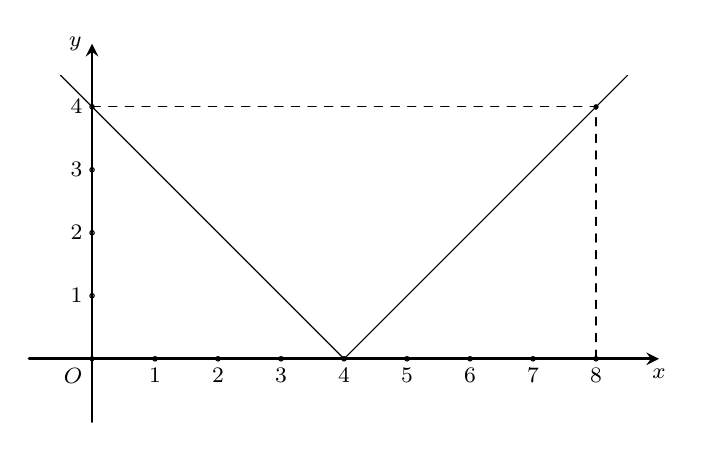
\begin{tikzpicture}[>=stealth,line join=round,line cap=round,font=\footnotesize,scale=0.8]
				\draw[->,line width = 1pt] (-1,0)--(9,0) node[below]{$x$};
				\fill (0,0) node[below left]{$O$} circle (1.2 pt);
				\draw[->,line width = 1pt] (0,-1) --(0,5) node[left]{$y$};
				\foreach \x in {1,2,3,4,5,6,7,8}{
					\draw (\x,0) node[below]{$\x$} circle (1pt);
				}
				\foreach \x in {1,2,3,4}{
					\draw (0,\x) node[left]{$\x$} circle (1pt);
				}
				\draw[dashed] (0,4)--(8,4)--(8,0);
				\draw [domain=-0.5:4, samples=100] %
				plot (\x, {(-1*(\x)+4)});
				\draw [domain=4:8.5, samples=100] %
				plot (\x, {((\x)-4)});
				\fill (8,4) circle(1.2pt);
		\end{tikzpicture}
		\end{center}
	}
	\loigiai{
		\begin{itemchoice}
			\itemch \textbf{Đúng}. Vì hàm số $f(x) = |x - 4|$ hoàn toàn xác định, do đó có tập xác định $\mathscr{D} = \mathbb{R}$.
			\itemch \textbf{Sai}. Vì $f(x) = |x - 4|$ nên $f(x) = \heva{&x - 4 &\text{ khi } x < 4\\&-x + 4 &\text{ khi } x \geq 4}$
			\itemch \textbf{Sai}. Với mọi $x_1$, $x_2 \in (4;+\infty)$ và $x_1 > x_2$, ta có
			$$ f(x_1) - f(x_2) = \left(x_1 - 4\right) - \left(x_2 - 4\right) = x_1 - x_2 > 0. $$
			Do đó $f(x_1) > f(x_2)$ nên hàm số đã cho đồng biến trên $(4;+\infty)$.\\
			Với mọi $x_1$, $x_2 \in (-\infty;4)$ và $x_1 > x_2$, ta có
			$$ f(x_1) - f(x_2) = \left(-x_1 + 4\right) - \left(-x_2 + 4\right) =  -\left(x_1 - x_2\right) < 0. $$
			Do đó $f(x_1) < f(x_2)$ nên hàm số đã cho nghịch biến trên $(-\infty;4)$.
			\itemch \textbf{Đúng}. Vì $f(x) = \heva{&x - 4 &\text{ khi } x < 4\\&-x + 4 &\text{ khi } x \geq 4}$ nên đồ thị của hàm số đã cho là
			\begin{center}
				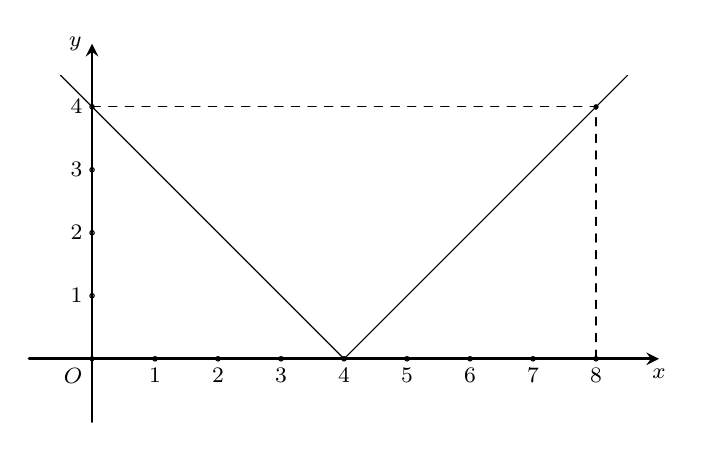
\begin{tikzpicture}[>=stealth,line join=round,line cap=round,font=\footnotesize,scale=0.8]
					\draw[->,line width = 1pt] (-1,0)--(9,0) node[below]{$x$};
					\fill (0,0) node[below left]{$O$} circle (1.2 pt);
					\draw[->,line width = 1pt] (0,-1) --(0,5) node[left]{$y$};
					\foreach \x in {1,2,3,4,5,6,7,8}{
						\draw (\x,0) node[below]{$\x$} circle (1pt);
					}
					\foreach \x in {1,2,3,4}{
						\draw (0,\x) node[left]{$\x$} circle (1pt);
					}
					\draw[dashed] (0,4)--(8,4)--(8,0);
					\draw [domain=-0.5:4, samples=100] %
					plot (\x, {(-1*(\x)+4)});
					\draw [domain=4:8.5, samples=100] %
					plot (\x, {((\x)-4)});
					\fill (8,4) circle(1.2pt);
				\end{tikzpicture}
			\end{center}
		\end{itemchoice}
	}
\end{ex}
\Closesolutionfile{ans}
%\inputansbox[2]{2}{ans/answer.tex}



\begin{center}
	\textbf{PHẦN 3 - TỰ LUẬN}
\end{center}
\setcounter{ex}{0}
%-----Câu 1
\begin{ex}%[0D2V2-3]%[Dự án đề kiểm tra Toán 10 GKI NH24-25-Trung Kiên]%[THPT Nguyễn Thị Minh Khai - Tp Hồ Chí Minh]
	Người ta dự định dùng hai loại nguyên liệu $K$, $P$ để sản xuất ít nhất $72$ kg sản phẩm loại $I$ và $80$ kg sản phẩm loại $II$. Từ mỗi tấn nguyên liệu $K$ giá $4$ triệu đồng, có thể sản xuất được $24$ kg sản phẩm loại $I$ và $40$ kg sản phẩm loại $II$. Từ mỗi tấn nguyên liệu $P$ giá $3$ triệu đồng, có thể sản xuất được $36$ kg sản phẩm loại $I$ và $20$ kg sản phẩm loại $II$. Hỏi phải dùng bao nhiêu tấn nguyên liệu mỗi loại để chi phí mua nguyên liệu là ít nhất? Biết rằng cơ sở cung cấp nguyên liệu chỉ có thể cung cấp tối đa $3$ tấn nguyên liệu loại $K$ và $4$ tấn nguyên liệu loại $P$.
	\loigiai{
		Gọi $x$, $y$ (tấn) lần lượt là số tấn nguyên liệu loại $K$ và $P$ cần mua. Khi đó $x \ge 0$, $y \ge 0$.\\
		Chi phí để mua $x$ tấn nguyên liệu $K$ và $y$ tấn nguyên liệu $P$ là $F(x;y)=4x+3y$ (triệu  đồng).\\
		Vì cơ sở cung cấp nguyên liệu chỉ có thể cung cấp tối đa $3$ tấn nguyên liệu loại $K$ và $4$ tấn nguyên liệu loại $P$ nên $x \le 3$, $y \le 4$.\\
		Vì cần sản xuất ít nhất $72$ kg sản phẩm loại $I$ và $80$ kg sản phẩm loại $II$ nên $24x+36y \ge 72$, $40x+20y \ge 80$.\\
		Từ đó ta thu được hệ bất phương trình sau:
		$$\heva{&0\le x \le 3\\&0\le y \le 4\\&24x+36y \ge 72\\&40x+20y \ge 80} \Leftrightarrow \heva{&0\le x \le 3\\&0\le y \le 4\\&2x+3y \ge 6\\&2x+y \ge 4.}$$
		Biểu diễn miền nghiệm của hệ bất phương trình trên mặt phẳng tọa độ, miền nghiệm là phần trong của tứ giác $ABCD$ (kể cả các cạnh của tứ giác) với $A(0;4)$, $B(3;4)$, $C(3;0)$ và $D(1{,}5;1)$.
		\begin{center}
			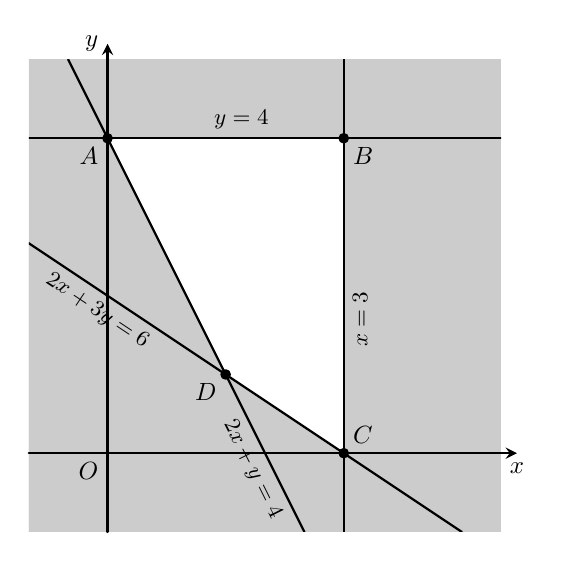
\begin{tikzpicture}[line join=round, line cap=round,>=stealth,thick]
				\tikzset{every node/.style={scale=0.9}}
				\begin{scope}
					\clip (-1,-1) rectangle (5,5);
					\fill[gray!40] (-5,5.33)--(-5,-2)--(6,-2)--cycle;
					\fill[gray!40] (-2,8)--(-2,-8)--(6,-8)--cycle;
					\fill[gray!40] (3,-1)--(5,-1)--(5,5)--(3,5)--cycle;
					\fill[gray!40] (-1,4)--(-1,5)--(5,5)--(5,4)--cycle;
					\fill[gray!40] (0,-1)--(-1,-1)--(-1,5)--(0,5)--cycle;
					\fill[gray!40] (-1,0)--(-1,-1)--(5,-1)--(5,0)--cycle;
					\draw (-4.5,5)--(4.5,-1) node [pos=0.5, below, sloped] {\small $2x+3y=6$};
					\draw (-0.5,5)--(2.5,-1) node [pos=0.85, below, sloped] {\small $2x+y=4$};
					\draw (3,-1)--(3,5) node [pos=0.45, below, sloped] {\small $x=3$};
					\draw (-1,4)--(5,4) node [pos=0.45, above, sloped] {\small $y=4$};
				\end{scope}
				\draw[->] (-1,0)--(5.2,0) node[below]{$x$};
				\draw[->] (0,-1)--(0,5.2) node[left]{$y$};
				\draw (0,0) node[below left]{$O$};
				\draw[fill=black] (0,4)circle(1.5pt) node[below left]{$A$}
				(3,4)circle(1.5pt) node[below right]{$B$}
				(3,0)circle(1.5pt) node[above right]{$C$}
				(1.5,1)circle(1.5pt) node[below left]{$D$}
				;
			\end{tikzpicture}
		\end{center}
		Ta có $F(0;4)=12$, $F(3;4)=24$, $F(3;0)=12$ và $F(1{,}5;1)=9$. Nên giá trị nhỏ nhất cần tìm là $F(1{,}5;1)=9$.\\
		Vậy dùng $1{,}5$ tấn nguyên liệu loại $K$ và $1$ tấn nguyên liệu loại $P$ thì chi phí mua nguyên liệu là ít nhất.
	}
\end{ex}

%-----Câu 2
\begin{ex}%[0H5V3-6]%[Dự án đề kiểm tra Toán 10 GKI NH24-25-Trung Kiên]%[THPT Nguyễn Thị Minh Khai - Tp Hồ Chí Minh]
	Cho tam giác $ABC$ có $AM$ là trung tuyến và $D$ là trung điểm của $AM$. 
	\begin{enumerate}
		\item Chứng minh $2\overrightarrow{DA}+\overrightarrow{DB}+\overrightarrow{DC}=\overrightarrow{0}$.
		\item Lấy điểm $E$ đối xứng với $A$ qua $B$ và điểm $F$ trên cạnh $AC$ thỏa mãn $5AF=2FC$. Chứng minh ba điểm $E$, $D$, $F$ thẳng hàng.
	\end{enumerate}
	\loigiai{
		\begin{center}
			\begin{tikzpicture}[scale=0.8,>=stealth, font=\footnotesize, line join=round, line cap=round]
				\draw
				(0,0) coordinate (B)
				--(4,0) coordinate (C)
				--(1,2.5) coordinate (A)--cycle
				(A)--($(B)!0.5!(C)$) coordinate (M)
				($(A)!0.5!(M)$) coordinate (D)
				(B)--($(A)!2!(B)$) coordinate (E)
				($(A)!2/7!(C)$) coordinate (F)--(E)
				;
				
				\foreach \x/\g in {B/180,C/0,A/90,M/-90,D/180,E/180,F/30}{\draw[fill=black] (\x) circle(1pt)+ (\g:0.3)node{$\x$};} 
			\end{tikzpicture}
		\end{center}
		\begin{enumerate}
			\item Vì $M$ là trung điểm $BC$ nên $\overrightarrow{DB}+\overrightarrow{DC}=2\overrightarrow{DM}$. Do đó
			$$2\overrightarrow{DA}+\overrightarrow{DB}+\overrightarrow{DC}=2\overrightarrow{DA}+2\overrightarrow{DM} = 2\left(\overrightarrow{DA}+\overrightarrow{DM}\right)=2\overrightarrow{0}=\overrightarrow{0}.$$
			\item Ta có 
			\begin{align*}
				\overrightarrow{ED}	&=\overrightarrow{EA}+\overrightarrow{AD}\\
				&=-2\overrightarrow{AB}+\dfrac{1}{2}\overrightarrow{AM}\\
				&=-2\overrightarrow{AB}+\dfrac{1}{4}\left(\overrightarrow{AB}+\overrightarrow{AC}\right)\\
				&=-\dfrac{7}{4}\overrightarrow{AB}+\dfrac{1}{4}\overrightarrow{AC}.
			\end{align*}
			Tương tự $\overrightarrow{EF}=\overrightarrow{EA}+\overrightarrow{AF}
			=-2\overrightarrow{AB}+\dfrac{2}{7}\overrightarrow{AC}$.
		\end{enumerate}
		Do đó $\overrightarrow{EF}=\dfrac{8}{7}\overrightarrow{ED}$.\\
		Vậy $E$, $D$, $F$ thẳng hàng.
	}
\end{ex}

